\section{File dropping launching}

\begin{frame}
 \begin{itemize}
  \item Problem: downloading files from a FTP server and processing them with Spring Batch
  \item Solution: use Spring Integration to poll the FTP server and trigger Spring Batch accordingly
 \end{itemize}
\end{frame}

\begin{frame}
 \frametitle{Using Spring Integration for transfer and triggering}
 \begin{center}
  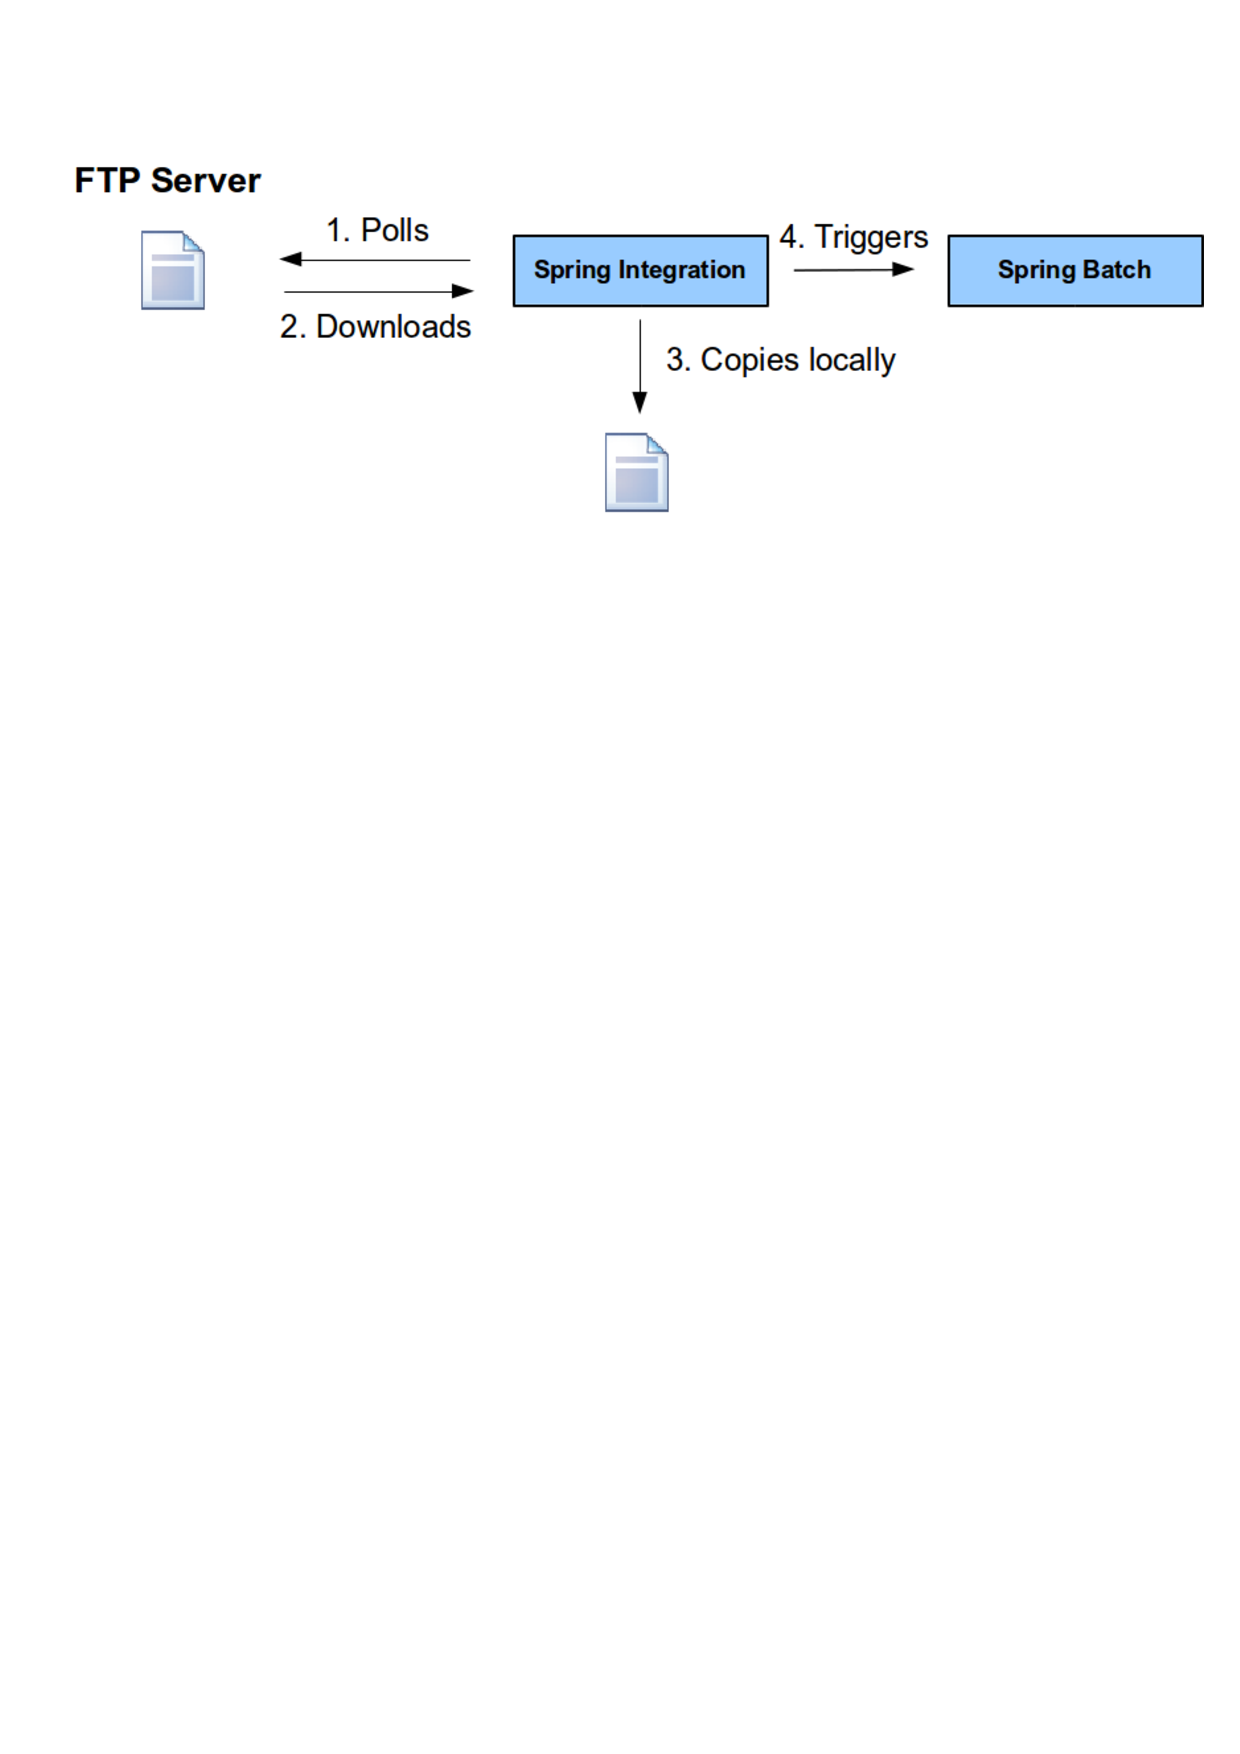
\includegraphics[width=10cm]{figures/spring-integration-ftp-poller.pdf}
 \end{center}
\end{frame}


\begin{frame}[fragile]
 \frametitle{The launching code}
 \begin{javacode}
public class FileContactJobLauncher {

  public void launch(File file) throws Exception {
      JobExecution exec = jobLauncher.run(
        job, 
        new JobParametersBuilder()
          .addString("input.file", "file:"+file.getAbsolutePath())
          .toJobParameters()
      );
  }

}  
 \end{javacode}

 \begin{itemize}
  \item The \code{File} is the local copy
 \end{itemize}
\end{frame}


\begin{frame}[fragile]
 \frametitle{Listening to the FTP server}
 \begin{xmlcode}
<int:channel id="fileIn" />

<int-ftp:inbound-channel-adapter local-directory="file:./input" 
    channel="fileIn" session-factory="ftpClientFactory" 
    remote-directory="/" auto-create-local-directory="true">
  <int:poller fixed-rate="1000" />
</int-ftp:inbound-channel-adapter>

<bean id="ftpClientFactory"
      class="o.s.i.ftp.session.DefaultFtpSessionFactory">
  <property name="host" value="localhost"/>
  <property name="port" value="2222"/>
  <property name="username" value="admin"/>
  <property name="password" value="admin"/>
</bean>
 \end{xmlcode}
\end{frame}

\begin{frame}[fragile]
\frametitle{Calling the launcher on an inbound message}
\begin{xmlcode}
<int:channel id="fileIn" />

<int:service-activator input-channel="fileIn">
  <bean 
    class="c.z.w.springbatch.integration.FileContactJobLauncher">
    <property name="job" ref="fileDroppingLaunchingJob" />
    <property name="jobLauncher" ref="jobLauncher" />
  </bean>
</int:service-activator>
 \end{xmlcode}
\end{frame}

\begin{frame}
 \frametitle{Going further...}
 \begin{itemize}
  \item Checking Spring Integration connectors
  \begin{itemize}
   \item Local file system, FTPS, SFTP, HTTP, JMS, etc.
  \end{itemize}
  \item Checking operations on messages
  \begin{itemize}
   \item Filtering, transforming, routing, etc.
  \end{itemize}
 \end{itemize}
\end{frame}

